\chapter{Introduction}
\label{ch1}

%%%%% https://cerncourier.com/a/pushing-the-precision-frontier/
% https://home.cern/news/news/physics/why-precision-luminosity-measurements-matter


\section{Particle Physics and the Standard Model}

Elementary particle physics is the study of the particles at the most fundamental level, the constituents of the universe as well as the interactions between them which are called, electromagnetic force, nuclear weak force and nuclear strong force and there is also the gravity force but this one doesn't have a satisfactory quantum theory for it. Each of these forces are mediated by exchange particles, in the case of the electromagnetic force the mediator is the photon, for the strong force the gluons, for the weak force the bosons W and Z and for the gravity we have the hypothetical graviton.  \cite{Griff}  

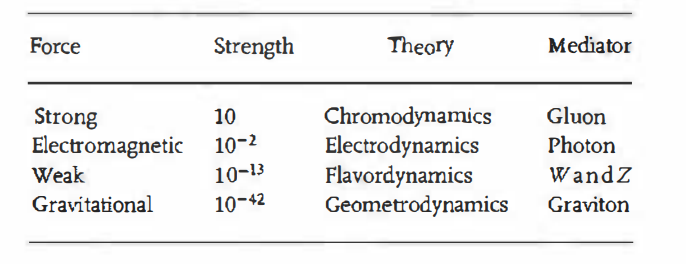
\includegraphics[scale=1]{table1.png}
\caption{Forces magnitude compared}

Each of these forces have a mathematical description for the physical systems of these interactions using the Quantum Field Theory (QFT). The one that describes systems under the electromagnetic force is called Quantum Electrodynamics (QED) this force dictates the electronic structure of atoms being the low energy manifestation of the electromagnetic theory. For the strong force Quantum Chromodynamics (QCD) is the fundamental theory of strong interactions, this force is responsible of maintaining protons and neutrons together in the atomic nucleus. For the weak interactions there is no particular name in the same way as the previous two, this force is is carried by all quarks and leptons and is responsible for the $\beta$ Decay of some radioactive isotopes and nuclear processes of the sun. \cite{mppthomson}   


Almost all the physical phenomena can be explained with only the electron, the electron neutrino, the proton and the neutron interacting with the electromagnetic force, the strong force and the weak one. When higher levels of energy are present new particles are observed, all of this is known as the elementary particles which are embodied in the standard model of particle physics that is by far the best theorical model that describes interaction of this elementary particles. Is divided into two categories the bosonic sector and the fermionic sector.  \cite{mppthomson}   

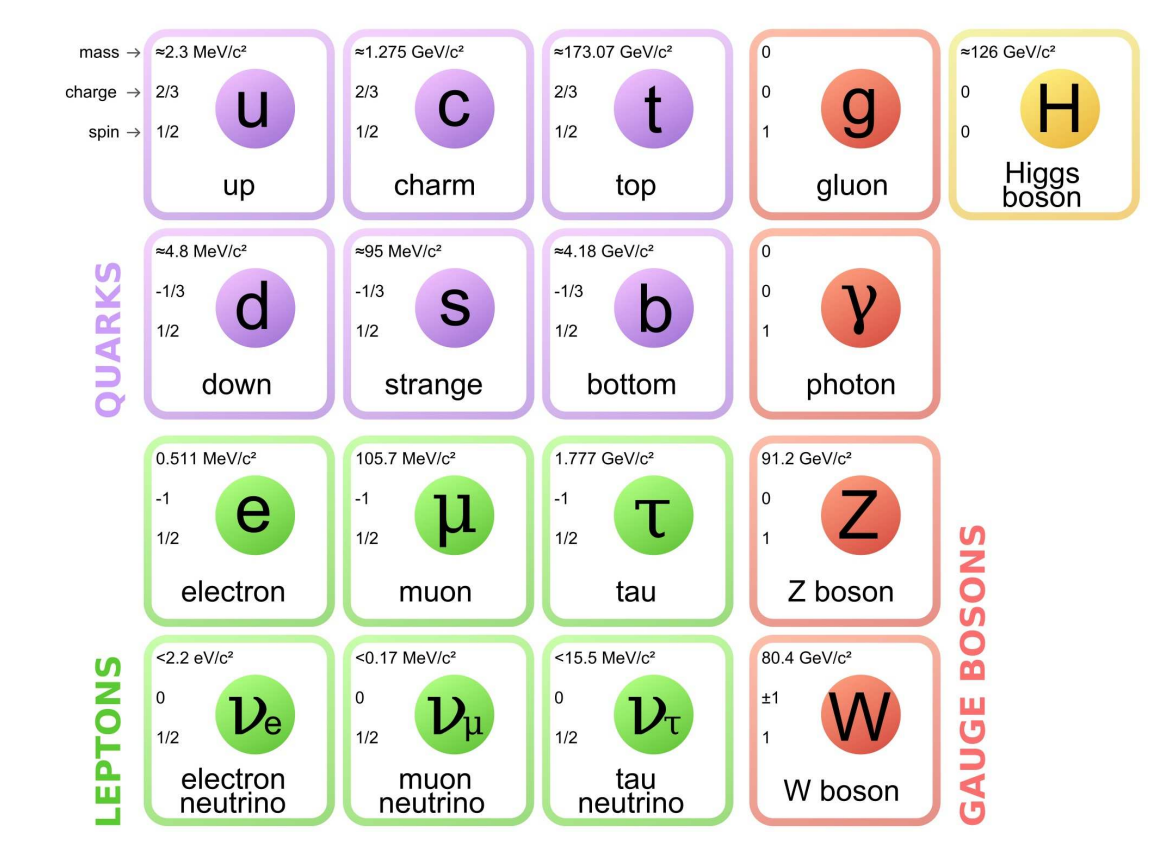
\includegraphics[scale=0.7]{sm.png}

The fermionic sector contains particle the particles that make up all known matter in the universe and is divided into the leptons and the quarks, both of this particles are divided into three generations, each generation being heavier than the one before. For the leptons we have electron and Its neutrino for the first generation, the second generation is. the $\mu$ and Its neutrino and the third one is the $\tao$ with Its neutrino. In the case of quarks we have the quark up and the quark down for the first generation, the second generation que have the quark charmd and the quark strange and for the third generation que have the quark top and the quark bottom. The bosons are the mediator particles called the gauge bosons already mentions, the photon, the gluon, the bosons $W\pm$ and the boson Z. There is also de Higgs bosson, which is the last gauge bossons and It's the responsible to give mass to the other SM particles  


One of the main sources to obtain elementary particles is particle accelerators, in this you accelerate a particle into high energy and smash them with a target, with the proper  arrangements of magnets you can study the debris from the collision, for more heavy particles you need higher level of energy to the collision.

\section{Large Hadron Collider}

The Large Hadron Collider (LHC) is the biggest and powerful particle accelerator in the world at this moment, It is a 27 kilometers ring of superconducting magnets, this magnets boost the particles energies to obtain speeds that are close to the light speed before collisions. These particles are introduced as to the accelerator as particles beams this beams travel in opposing directions in tubes that are kept at ultrahigh vacuum, with the help of a electromagnetic field made by the electromagnets operating in superconduct state at low temperatures thanks to liquid helium this particles are guided across the whole accelerator. \cite{LHC}


 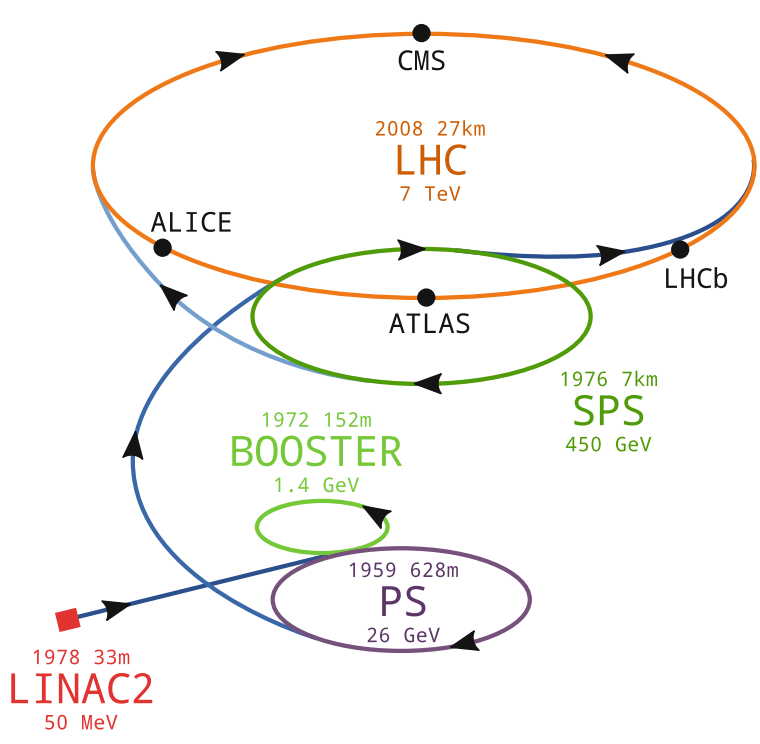
\includegraphics[scale=0.35]{LHC.png}

The LHC is part of an accelerator complex in CERN that is a succession of different machines that increase the energy of the beam of particles before passing into the next one on the sequence the particles at last are introduced on the LHC which is the last element in the sequence. The particles start at the linear accelerator 4 (Linac4) which is the source of the protons beams, it accelerates the particles in this case negative hydrogen ions to 160 MeV to enter the Proton Synchroton Booster (PSB), this is were the hydrogen loses Its two electrons leaving only protons and accelerating the beam to 2 GeV  and then are injected into the Proton Synchroton (PS), in where the protons are accelerated up to 26 GeV and then they are sent into the Super Proton Synchroton (SPS) here they are accelerated up to 450 GeV and then they're finally introduced into two beams pipes on the LHC, it takes about 4 minutes and 20 seconds to fill the LHC rings reaching energies up to 6.5 TeV, there are 4 collisions points where the detectors are located Alice, Atlas, CMS and LHCb, in the collision the total energy is of 13.6 TeV. \cite{LHCII}

The LHC has been working since 2009 with the discovery of the Higgs Boson on 2012 and looking for new physics It has been working on different periods called Runs, Run 1 was on the period of (2009-2013), Run 2 was on (2015-2018), Run 3 is currently on going since 2022. 



\section{Luminosity}

The performance of a collider is determined by the beam energy and the luminosity, the luminosity is a key parameter in particle colliders is a quantity that measures the ability of a particle accelerator to produce a required number of interactions and is given by: \cite{Lum} 

$\frac{dR}{dt} = \mathcal{L} \cdot \sigma_{p} $ 

In which $\frac{dR}{dt}$ is the number of events per second, the $\simga_{p}$ is the cross section and $\matchcal{L}$ the instantanious luminosity luminosity. The unity of $\mathcal{L}$ is  $cm^{-2} s^{-1}$ a higher luminosity means greater probability that the particles will collide and produce the desired interactions, luminosity can be increased then in two ways, packing more particles into the beams or focusing this beams more.  

 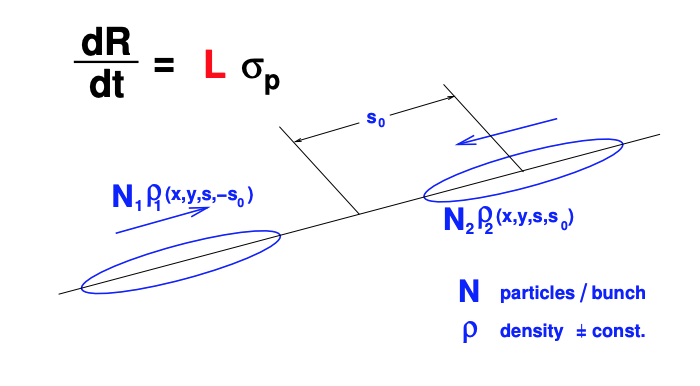
\includegraphics[scale=0.80]{lumii.png}


To compute the luminosity of two there is a few things that need to be taken in consideration. First the density distribution of each beam in the transverse and longitudinal plane, with the. two beams moving towards each other, the position and the time as the cross each other also need to be considered and calling the distance to the collision point $s_{0}$. In principle each of the distributions is different the overlap integral can be written as follow:

 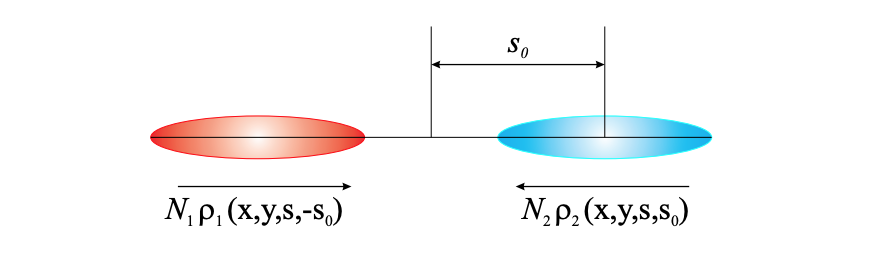
\includegraphics[scale=0.80]{lumi.png}


$ N_{1}N{2}fN_{b} K \int \int \int^{\infty}_{-\infty}  \rho_{1} (x,y,s,s_{0}) \rho_{x}(x,y,s,s_{0})  dxdydsds_{0}  $

With N1 and N2 being the bunch intensitie, f the revolution frecuency, $N_{b}$ the number of colliding bunches, $\rho_{1}$ and $\rho_{2}$ time dependent beam density distribution functions and K being the Kinematic factor defined as: 

$K = sqrt{(v_{1} - x_{2})^{2} - \frac{(v_{1} x v_{2})^{2}}{c^{2}} }

So now assuming that the velocity on the beams is $v1 = -v2$ and the densities are uncorrelated in all planes the overlap integral takes the form of: \cite{Lumvdm}

$ 2N_{1}N{2}fN_{b} \int \int \int^{\infty}_{-\infty}  \rho_{1x} (x) \rho_{1y}(y) \rho_{1s} (s-s_{0}) \rho_{2x}(x) \rho_{2y}(y) \rho_{2s} (s+s_{0}) dxdydsds_{0}  $

For solving this integral one should known all distributions and an analytical solutions might not be possible and numerical numerical integration might be required.


The instantaneous luminosity is important  but the final important number is called integrated luminosity. The integrated luminosity considers the total number of events during a data period is defined as: 

$ L_{int} = \int L (t') dt' $

it is related directly to the number of observed events 

$\mathcal{L}_{int} \cdot \sigma_{p} =$ number of events of interest 

There have been different luminosities reached on the LHC for the Run 1 a luminosity of $0.77 x 10^{34}$ was reached and a integrated luminosity of 25 $fb^{-1}$  with a precision of 2.0\% for the first part and second part of the Run 2 the luminosity measured was of 38.4 $fb^{-1}$ with a precision of 1.3\% and 78$fb^{-1}$ respectively\cite{LHClum}.  The following image show shows the integrated luminosity for the CMS experiment on different years.  

 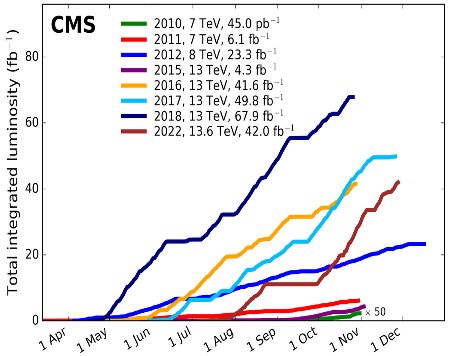
\includegraphics[scale=1.25]{integratedlum.png}

